\documentclass[12pt]{article}

\usepackage[american]{babel}
\usepackage[utf8]{inputenc}
\usepackage[T1]{fontenc}
\usepackage[english=american]{csquotes}

\setlength{\textfloatsep}{22pt plus 1.0pt minus 2.0pt}

\usepackage{graphicx}
\usepackage{caption}
\captionsetup{font=small} % fa els peus de pàgina més petits

\usepackage[style=apa, backend=biber, natbib=true]{biblatex}
\addbibresource{C:/Users/aleja/Bibtex/library.bib}
\addbibresource{misc.bib}

%\usepackage[nospace]{varioref}
\usepackage{hyperref}
\usepackage{cleveref}
%\usepackage[T1]{tipa} %notació fonètica IPA


\setlength{\parskip}{1em}

\usepackage{titling}
\setlength{\droptitle}{-10em} 
\author{Alejandro García Matarredona}
\title{Assignment 1. Introduction to the Hewa language}
\date{September 20, 2021}

\begin{document}

\maketitle

%General info about the language
%Previous documentation: Klamer wordlist


Hewa (not to be confused with a language of the same name spoken in Papua New Guinea, ISO 639-3: ham) is a language variety spoken in the village of the same name, in the eastern part of the island of Flores in eastern Indonesia. A few documents exist on Hewa. There is one wordlist by Marian Klamer \citep{klamer_2015}, as well as a few materials from Hanna Fricke, among them a sketch grammar \citep{Fricke2014} and a dictionary \citep{fricke_2015}. It is considered a dialect of the better documented Sika language (ISO 639-3: ski), spoken along eastern Flores (see \cref{fig:langmap}), and which belongs to the Central-Eastern Malayo-Polynesian group in the Austronesian family \citep{Lewis1995}. Sika is estimated to have approximately 175,000 speakers (ibid.).

%Hewa = Sika Krowe??!!?
%Maybe include typological info on the language(extra)

\begin{figure}[h]

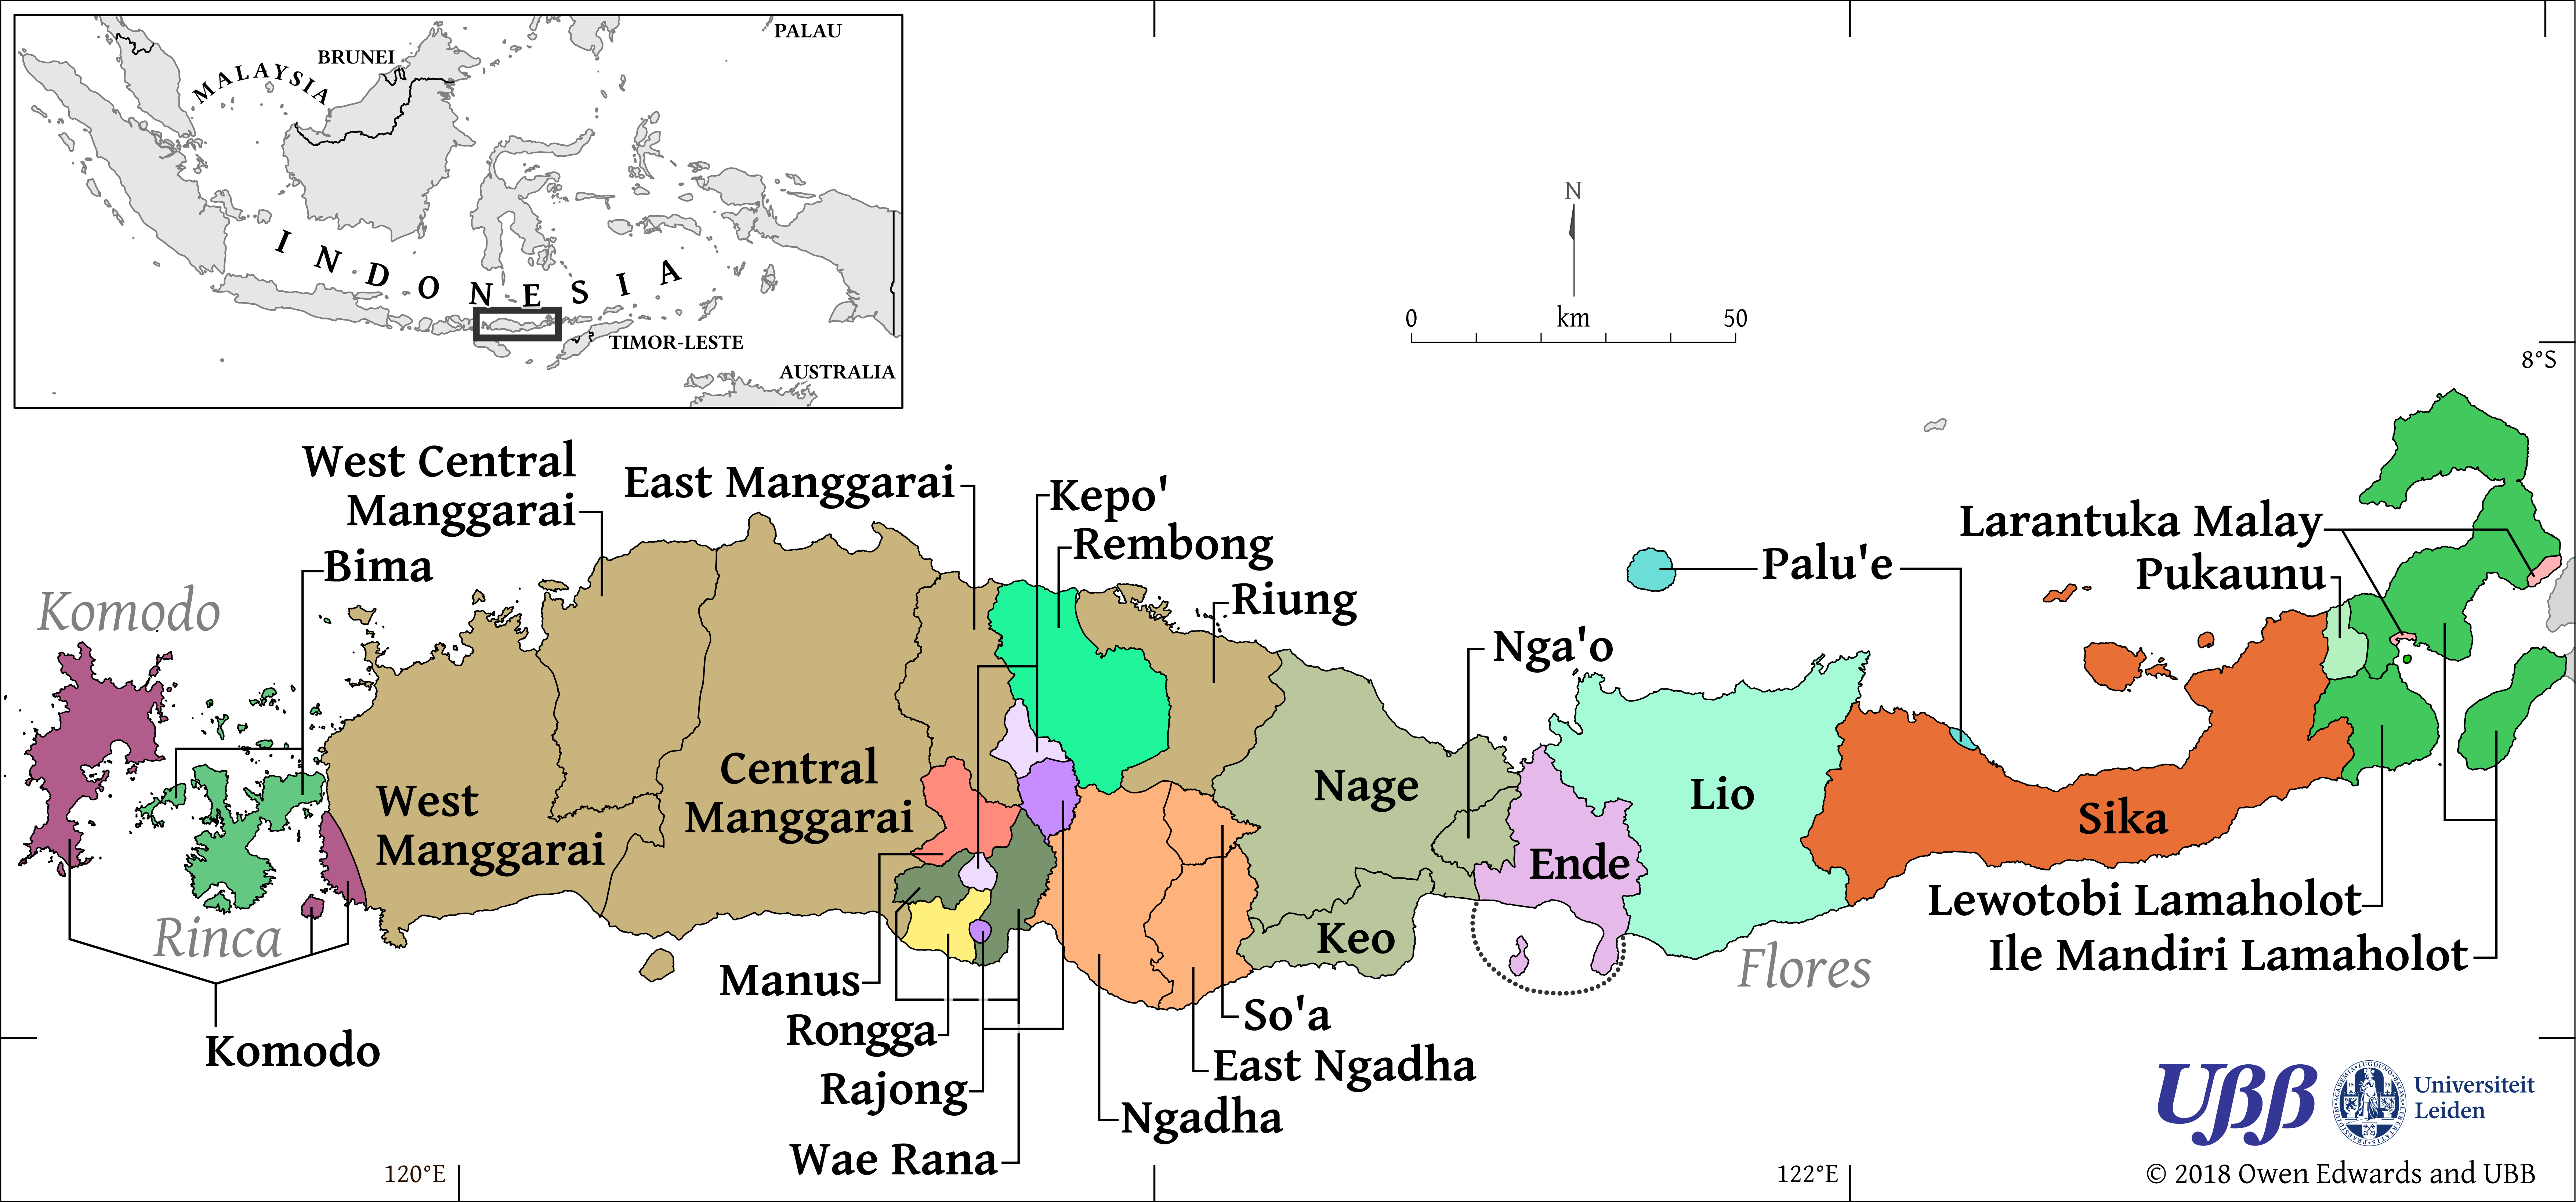
\includegraphics[width=0.9\linewidth] {Images/flores_languages__inset_.png}

\caption{Language map of the island of Flores \citep{edwards_ubb_2018}}
\label{fig:langmap}
%where in the world is the region in the map? Need one with a larger scope
\end{figure}

%Consultant and fieldwork

The present documentation project has taken place during a course in Field Methods as part of the MA Linguistics programme at Leiden University in the fall of 2021. Our language consultant is Eman, a 30 year-old male native speaker of Hewa who also speaks Indonesian and English and who is also an MA student at the University. The recordings were made in the classroom during teaching hours as well as during private meetings with the consultant.

%where has he lived? has he spent a significant amount of time outside his village, where people speak other languages? Does he speak the language nowadays?

%What equipment are we using? Vide and audio; external microphone
%Format of the data: mp4 files and WAV files

\printbibliography

\end{document}